\documentclass[11pt,a4paper]{article}
\usepackage[utf8]{inputenc}
\usepackage[T1]{fontenc}
%\usepackage{gentium}
\usepackage{mathptmx} % Use Times Font

\usepackage{graphicx} % Required for including pictures
\usepackage{hyperref} % Format links for pdf
\usepackage{biblatex}
\addbibresource{references.bib}
\usepackage{booktabs} % Used so that tables generated by pandas
                      % to_latex() work correctly

\frenchspacing % No double spacing between sentences
\usepackage[margin=1in]{geometry}

\usepackage[all]{nowidow} % Tries to remove widows
\usepackage[protrusion=true,expansion=true]{microtype} % Improves typography, load after fontpackage is selected

\usepackage{lipsum} % Used for inserting dummy 'Lorem ipsum' text into the template

\title{descriptive title about chess}
\author{Leon Lee and Lila Marshman}

\begin{document}

\maketitle

%% INSTRUCTIONS:
%%
%% 1. Create your own copy of this Overleaf project. You can either edit your report
%% using:
%%
%%    a. Overleaf professional, a collaborative LaTeX editor. You can click
%%       "Copy Project" from the Overleaf menu to create a version where you have
%%       read and write permissions. See the following for documentation:
%%       https://www.overleaf.com/edu/edinburgh and
%%       https://uoe.sharepoint.com/:f:/r/sites/digitalskillsandtraining/Shared%20Documents/LaTeX/LaTeX%20for%20Beginners%20using%20Overleaf?csf=1&web=1&e=cPqTI3
%%
%%    b. A LaTeX editor on your PC. For this option, you can download the source
%%       of this project as a zip (via the Overleaf menu).
%% 
%% 2. Please rename this file fds-project-option-1.tex, 
%% fds-project-option-2.tex, or fds-project-option-3.tex, depending on
%% which project option you are doing. When you submit, please submit
%% the PDF file with the corresponding name.
%% 
%% 3. Please keep the section and paragraph headings as they
%%    are. You should delete all the text within the headings, e.g.
%%    the text that says "What is the area of this data science
%%    study, and why is it interesting to investigate" and the
%%    bullet points. Keeping the headings makes the report a lot
%%    easier for the markers to read, and making things easy for
%%    markers is always beneficial.
%%
%% 4. The word limit for the Overview section is mandatory. For the
%% other sections word limits are suggested.
%%
%% 5. The page limits must be strictly adhered to, and depend on if
%% you are working individually, in pairs or in threes:
%%
%%   - Individual: 6 pages 
%%   - Pairs: 8 pages 
%%   - Threes: 10 pages 
%%

\section{Overview}
% 250 words maximum

Visualisations of ...
Statistical techniques used ...

\section{Introduction}
% Suggested 400 words

\paragraph{Context and motivation}

Online chess has become increasingly popular, with website Chess.com hosting an average of x [Lila find and cite] games every day. Users may play with friends or strangers, and a wide variety of chess variants and time-controls are available to play with. It's rise in popularity follows the increase in free time during the COVID-19 pandemic lockdowns, popularity of Netflix's show 'The Queen's Gambit', and world-ranking players streaming the game on Twitch \cite{The2020ChessBoom} With a sudden increase in online players comes an increase in publicly available game data. This provides opportunity for investigation into player's strengths, measured by ELO (a number corresponding to skill level).

[Lila where? to put this bit:]

This report studies a dataset of 60,000 games, analysing the impact a difference in ELO (score related to playing ability in chess) makes on the outcome of a game. We also consider whether ELO may be predicted from a player's response to an 'en passant' move.

\paragraph{Previous work}

Brief description of any previous work in this area (e.g., in the
media, or scientific literature or blogs).

An article in the literature found [Lila put what it found] about the ELO \cite{HowMuchDoesEloMatter}.
There is no literature directly studying the relationship between a player's response to 'en passant' moves and their ELO.
\paragraph{Objectives}

% What questions are you setting out to answer?
Commonly, chess tactics are a way to gain an inherent advantage in the game state. Thus, a highly ranked chess player could plan ahead several moves just to obtain this state. Common tactics are ones that most players that are somewhat into chess will recognise as an advantageous move, but being able to consistently plan to apply the knowledge is what separates a good chess player from a great one. However, one exception to this is the move \textit{en-passant}. This is a far more situational tactic, and heavily relies on your opponent to move a certain way for a player to be able to utilise it. More importantly, often it does not leave the board in an advantageous state for the moving player. Due to this, compared to most other chess tactics, generally using en-passant will not be the optimal move. Therefore, if you are highly ranked and playing to win, chances are that you would not take it given the chance. However, in the chess scene, and especially in online chess which is where this dataset is sourced from, the move has gained a cult-like following. Since most people that are active in the online chess scene will be lower elo, we can use this fact to try and predict the elo of an individual player based on the chance they will take an en-passant, since we can assume that the higher the elo you are, the less likely to take it

\section{Data}
% Suggested 300 words

% Who created the dataset(s)?  How you have
% obtained it (e.g., file or web scraping), and do the T\&Cs allow you
% to use obtain the data for the project?

\paragraph{Data provenance}
We obtained our data from Kaggle.com \cite{Kaggle}, where they provided a dataset of over 60,000 games of chess taken from Chess.com. The terms and conditions on Chess.com state that you are not allowed to datamine[todo: cite chess.com t\&c], but in this case the dataset was extracted using the Chess.com API so it complies with their regulations.

% Description of the data, e.g. variables
% in each table, number of records.
\paragraph{Data description}
The dataset records 66879 games of chess that took place on Chess.com with varying game modes, time classes, and levels of players. The data is all in one file but the columns are effectively split up into two sections. The first are the main columns, while the final column is the PGN. The main columns include basic data i.e. the usernames and links of players, the ELO ratings of each player, the result of both players, the time control and time class, the rules the game was played on, and the final board state. On the other hand, the PGN (Portable Game Notation) is a column in a standard format to be easily read by other chess analysers. Thus it has a lot of the same information the previous fields do, but it also includes important information like the opening moves, and especially the last field which is a list of all the moves that took place during that game. Using the PGN we can simulate and replay exactly how the game was played, and analyse using that.

% How you have processed the dataset, e.g.,
% cleaning, removing missing values, joining tables.
\paragraph{Data processing}
The data was well set out, so it did not need much cleaning in terms of removing invalid entries or N/A values. However, since the dataset includes lots of different modes of games, some which are not standard chess, we removed them since they wouldn't be an accurate representation of an average chess game. One example of a chess variation is Chess960, where the starting positions of the pieces are randomised.
We also removed games where the game terminated early - either from timeout, resignation or other means. We used two filters, the first being to read the top row of the end-board, and if the pieces are laid out in the order "RNBKQBNR", that's an indicator that the game has not developed much since all the important pieces are in their starting place. Our second method was to filter out any games with less than 10 total moves (or 5 per player). We concluded that any games in these two categories would not be useful to the data analysis.

\section{Exploration and  analysis}
% Suggested 500 words for individual report; proportionately longer
% for group projects).

% 't' means "try to position at the top of the page"
\begin{figure}[t]
  \centering
  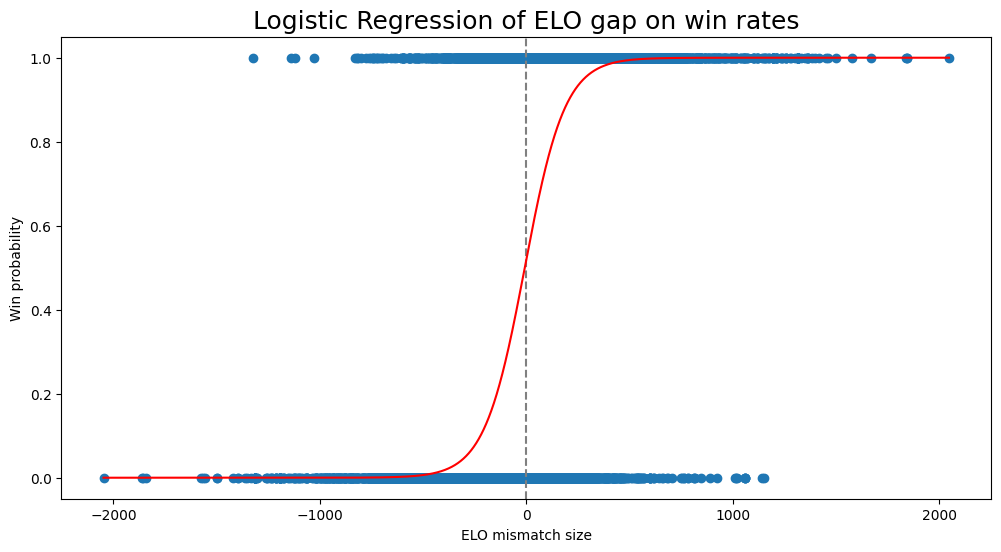
\includegraphics{report/images/log_regression.png}
  \caption{Each datapoint represents how many ELO points a player is than their opponent during a game, and whether they won (1) or lost (0). The standard logistic function is plotted in red.
  Demonstration figure. This caption explains more about the figure. Note that the font size of the labels in the plot is 9pt, which is obtained by the settings as shown in the Jupyter notebook.}
  \label{fds-project-template:fig:log_regression}
\end{figure}

% 'b' means "try to position at the bottom of the page"

\paragraph{Data Analysis}
We used logistic regression to investigate the association between the difference in player's ELO (a continuous predictor) and winning (a binary outcome, since draws or other indeterminate end-states are excluded).
A stratified sample of the dataset was made, proportionally sampling by 'time class' ('daily', 'rapid', 'blitz', 'bullet').
We found $\beta_{0}$ and $\beta_{1}$ to be $0.07679$ and $0.01028$ (5dp) respectively, thus can calculate the probability of a win is $\displaystyle\frac{1}{1+e^{\beta^{0}}}$.



You can use equations like this:
\begin{equation}
  \label{fds-project-template:eq:1}
  \overline{x} = \sum_{i=1}^n x_i
\end{equation}
or maths inline: $E=mc^2$. However, you do not need to reexplain techniques that you have learned in the course -- assume the reader understands linear regression, logistic regression K-nearest neighbours etc.  Remember to explain any symbols use, e.g.~``$n$ is the number of data points and $x_i$ is the value of the $i$th data point.''.

\section{Discussion and conclusions}
% Suggested 400 words.

\paragraph{Summary of findings}

\paragraph{Evaluation of own work: strengths and limitations}

\paragraph{Comparison with any other related work}
E.g. ``Anscombe has also demonstrated that many patterns of data can
have the same correlation coefficient'' \cite{anscombe1973graphs}.

Wikipedia can also be cited but it is better if you find the original
reference it for a particular claim in the list of references on the
Wikipedia page, read it, and cite it.

The golden rule is always to cite information that has come from other
sources, to avoid plagiarism \cite{wiki:plagarism}. \cite{HowMuchDoesEloMatter}

\paragraph{Improvements and extensions}


\printbibliography
\end{document}

% LocalWords:  lrrrrrrr ment Macduff Kemnay Ruchill FDS mc th fds
% LocalWords:  Anscombe